% Surabhi Jain
% UWP 101 Research Paper Draft 3

\documentclass{article}
\usepackage{changepage,multicol,tikz}
\usepackage[mathcal]{euscript}
\usepackage[backend=bibtex,sorting=none]{biblatex}
\usepackage[fontsize=9pt]{fontsize}
\usepackage[margin=1.5in]{geometry}

\title{\textbf{A Perspicuous Survey of \\ Zero-Knowledge Proofs}}
\author{Surabhi Jain}
\date{}
\addbibresource{research3.bib}

\begin{document}
\maketitle


\section{Introduction}

Since the time of Euclid, mathematical \textit{proofs}---logical arguments defending the truth of mathematical statements---have largely remained the same. These traditional proofs demonstrate to their receivers that the statements they concern are true, but they also divulge \textit{why} those statements are true. For thousands of years, no one considered whether there could be an alternative to this---but in 1985, that changed.

Indeed, 1985 was the year that Shafi Goldwasser, Silvio Micali, and Charles Rackoff wrote the seminal paper `The Knowledge Complexity of Interactive Proof Systems' (hereafter `Interactive Proof Systems'). Goldwasser, Micali, and Rackoff were cryptographers---scientists in the discipline of \textit{cryptography}, the study of secure communication in the presence of an adversary---and their paper introduced the concept of the \textit{zero-knowledge proof} (ZKP), an alternative type of proof.

Traditional, `true' proofs may follow a variety of structures. For example, the premises of the argument may be stated, and then it may be shown that the combination of these premises necessitates the truth of some given statement; alternatively, it may be shown that given the premises, the statement must be true because it is impossible for it to be false. All of these mathematical proofs, however, share the quality of establishing based on stated premises and through deductive reasoning---some series of logical inferences---that the statement in question must necessarily be true. In ZKPs, on the other hand, this reasoning remains a secret; indeed, the only new knowledge revealed to the receiver of a ZKP is that the statement being proven is in fact true \cite{GMR}.

For example, consider \textsc{Graph k-Coloring}, the problem of finding, given a graph---a set of `nodes' connected by `edges'---and some $k$, whether or not the nodes of the graph can be assigned $k$ colors in a manner such that that no connected nodes are the same color. Say that $k = 3$ and the graph is as displayed in I below. A true proof that this graph can be 3-colored would simply be the presentation of a valid 3-coloring of the graph, as in II. The terms of a ZKP, however, disallows the receiver of the proof to actually learn the 3-coloring. As such, a ZKP for the problem may go as follows. First, the creator of the proof creates a valid 3-coloring. They then `commit' it---by drawing it on a board and covering the nodes with Post-its, for example. The recevier may uncover any two nodes connected by an edge to ensure the validity of the coloring. Then, the creator draws and hides a different permutation, or `rotation', of the colors, and the receiver again may check any two connected nodes. This repeats until the receiver is satisfied that the 3-coloring is valid. This works because if the receiver checked every edge, then they could ensure that no two connected nodes are the same color, but since the colors are permuted after every check, it would be impossible for them to learn which unconnected nodes are the same color and reproduce the 3-coloring.

\begin{center}
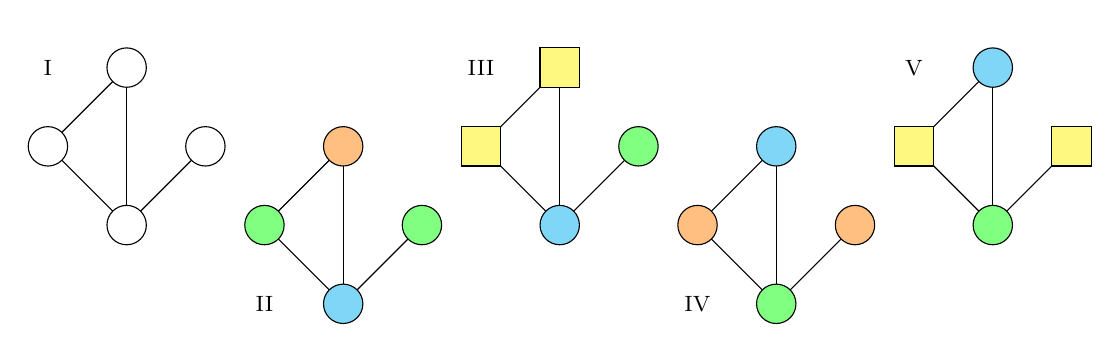
\begin{tikzpicture}
	\draw [] (1.25,3) -- (0.25,2);
	\draw [] (1.25,3) -- (1.25,1);
	\draw [] (2.25,2) -- (1.25,1);
	\draw [] (0.25,2) -- (1.25,1);

	\draw [] (4,2) -- (3,1);
	\draw [] (4,2) -- (4,0);
	\draw [] (5,1) -- (4,0);
	\draw [] (3,1) -- (4,0);

	\draw [] (6.75,3) -- (5.75,2);
	\draw [] (6.75,3) -- (6.75,1);
	\draw [] (7.75,2) -- (6.75,1);
	\draw [] (5.75,2) -- (6.75,1);

	\draw [] (9.5,2) -- (8.5,1);
	\draw [] (9.5,2) -- (9.5,0);
	\draw [] (10.5,1) -- (9.5,0);
	\draw [] (8.5,1) -- (9.5,0);

	\draw [] (12.25,3) -- (11.25,2);
	\draw [] (12.25,3) -- (12.25,1);
	\draw [] (13.25,2) -- (12.25,1);
	\draw [] (11.25,2) -- (12.25,1);

	\draw [color=white,text=black] (0,3) rectangle ++(0.5,0.5) node [] at (0.25,3) {\small I};
	\draw [fill=white] (1.25,3) circle (0.25);
	\draw [fill=white] (2.25,2) circle (0.25);
	\draw [fill=white] (1.25,1) circle (0.25);
	\draw [fill=white] (0.25,2) circle (0.25);

	\draw [color=white,text=black] (2.75,0) rectangle ++(0.5,0.5) node [] at (3,0) {\small II};
	\draw [fill=orange!50] (4,2) circle (0.25);
	\draw [fill=green!50] (5,1) circle (0.25);
	\draw [fill=cyan!50] (4,0) circle (0.25);
	\draw [fill=green!50] (3,1) circle (0.25);

	\draw [color=white,text=black] (5.75,3) rectangle ++(0.5,0.5) node [] at (5.75,3) {\small III};
	\draw [fill=yellow!50] (6.5,2.75) rectangle ++(0.5,0.5);
	\draw [fill=green!50] (7.75,2) circle (0.25);
	\draw [fill=cyan!50] (6.75,1) circle (0.25);
	\draw [fill=yellow!50] (5.5,1.75) rectangle ++(0.5,0.5);

	\draw [color=white,text=black] (8.25,0) rectangle ++(0.5,0.5) node [] at (8.5,0) {\small IV};
	\draw [fill=cyan!50] (9.5,2) circle (0.25);
	\draw [fill=orange!50] (10.5,1) circle (0.25);
	\draw [fill=green!50] (9.5,0) circle (0.25);
	\draw [fill=orange!50] (8.5,1) circle (0.25);

	\draw [color=white,text=black] (11,3) rectangle ++(0.5,0.5) node [] at (11.25,3) {\small V};
	\draw [fill=cyan!50] (12.25,3) circle (0.25);
	\draw [fill=yellow!50] (13,1.75) rectangle ++(0.5,0.5);
	\draw [fill=green!50] (12.25,1) circle (0.25);
	\draw [fill=yellow!50] (11,1.75) rectangle ++(0.5,0.5);
\end{tikzpicture} \\ \vspace{0.1in}
\noindent \textit{\small Image Source: Surabhi Jain}
\end{center}

Still, ZKPs may seem strange. In general, how can they be created? And what's the point of them, anyway? `Interactive Proof Systems' addresses both of these questions. Both answers are complicated, and have been further complicated after decades of following research. In brief, the paper's respective answers to these questions are through \textit{interactive proof systems}, and to construct \textit{secure cryptosystems}. But what do these answers mean? Each requires separate and careful attention.


\section{Interactive Proof Systems}

In `Interactive Proof Systems', Goldwasser, Micali, and Rackoff introduce, in addition to ZKPs, interactive proof systems (IPSs). IPSs are formal systems of communicating proofs that allow for interaction between a prover and a verifier, like the `creator' and `receiver' in the previously-described ZKP \cite{GMR}. The salient feature of such systems is that verifiers are `active', unlike the receivers of true proofs, which simply involve the presentation of inferences. IPSs were introduced as a way to convey ZKPs; to understand how they achieve their purpose, a more mathematical examination is necessary.

\begin{adjustwidth}{0.5in}{0in}
\subsection{The Turing Machine}

Many people are familiar with Alan Turing. Some know of his work as an early cryptographer in breaking the Enigma cipher in World War II. Fewer, however, know of his work as a mathematician in introducing the \textit{Turing machine}---and how it has contributed to modern cryptography.

In short, a Turing machine is a mathematical construct that makes computations by reading and writing on an infinitely long tape following a given set of instructions. A Turing machine in operation may be visualized as shown below. An input consisting of discrete symbols is written on the tape, and the machine head reads each symbol one-by- \vspace{-0.15in}

\begin{multicols}{2}
\noindent 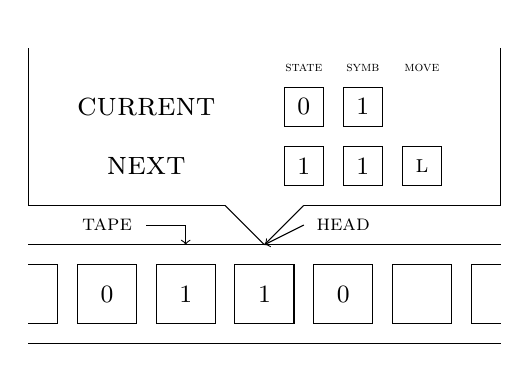
\begin{tikzpicture}
	\draw [] (3,2) -- (3,0);
	\draw [] (3,0) -- (0.5,0);
	\draw [] (0.5,0) -- (0,-0.5);
	\draw [] (0,-0.5) -- (-0.5,0);
	\draw [] (-0.5,0) -- (-3,0);
	\draw [] (-3,0) -- (-3,2);

	\draw [color=white,text=black] (-2.5,1) rectangle ++(2,0.5) node [] at (-1.5,1.25) {\textsc{\Large current}};
	\draw [color=white,text=black] (-2.5,0.25) rectangle ++(2,0.5) node [] at (-1.5,0.5) {\textsc{\Large next}};
	\draw [color=white,text=black] (0.25,1.625) rectangle ++(0.5,0.25) node [] at (0.5,1.75) {\textsc{\tiny state}};
	\draw [color=white,text=black] (1,1.625) rectangle ++(0.5,0.25) node [] at (1.25,1.75) {\textsc{\tiny symb}};
	\draw [color=white,text=black] (1.75,1.625) rectangle ++(0.5,0.25) node [] at (2,1.75) {\textsc{\tiny move}};
	\draw [] (0.25,1) rectangle ++(0.5,0.5) node [] at (0.5,1.25) {0};
	\draw [] (1,1) rectangle ++(0.5,0.5) node [] at (1.25,1.25) {1};
	\draw [] (0.25,0.25) rectangle ++(0.5,0.5) node [] at (0.5,0.5) {1};
	\draw [] (1,0.25) rectangle ++(0.5,0.5) node [] at (1.25,0.5) {1};
	\draw [] (1.75,0.25) rectangle ++(0.5,0.5) node [] at (2,0.5) {\textsc{l}};

	\draw [] (3,-0.5) -- (-3,-0.5);
	\draw [] (3,-1.75) -- (-3,-1.75);
	\draw [] (3,-0.75) -- (2.625,-0.75);
	\draw [] (2.625,-0.75) -- (2.625,-1.5);
	\draw [] (2.625,-1.5) -- (3,-1.5);
	\draw [] (1.625,-1.5) rectangle ++(0.75,0.75);
	\draw [] (0.625,-1.5) rectangle ++(0.75,0.75) node [] at (1,-1.125) {0};
	\draw [] (-0.375,-1.5) rectangle ++(0.75,0.75) node [] at (0,-1.125) {1};
	\draw [] (-1.375,-1.5) rectangle ++(0.75,0.75) node [] at (-1,-1.125) {1};
	\draw [] (-2.375,-1.5) rectangle ++(0.75,0.75) node [] at (-2,-1.125) {0};
	\draw [] (-3,-0.75) -- (-2.625,-0.75);
	\draw [] (-2.625,-0.75) -- (-2.625,-1.5);
	\draw [] (-2.625,-1.5) -- (-3,-1.5);

	\draw [->] (0.5,-0.25) -- (0,-0.5) node [] at (1,-0.25) {\textsc{\small head}};
	\draw [->] (-1.5,-0.25) -| (-1,-0.5) node [] at (-2,-0.25) {\textsc{\small tape}};

	\draw [color=white] (3,2.25) -- (-3,2.25);
\end{tikzpicture} \vspace{0.05in}
\noindent \begin{center} \textit{\small Image Source: Surabhi Jain} \end{center}

\noindent one. Encoded into the machine are a start state and instructions for changing the symbol in the current position, changing the state, and moving to the symbol on the left or right depending on the current state and symbol. Some states may be `accept' states or `reject' states; if the machine reaches a state of one of these types, then it halts computation.

Given some input on its tape, a Turing machine either runs forever, or it eventually halts. If it halts on an accept state, then the 
\end{multicols} \vspace{-0.15in}

\noindent input is `accepted' as being in the domain of the function that the Turing machine computes, and the final contents of the tape are its corresponding output. It has been shown that there exists a Turing machine for every computable function.
\end{adjustwidth} \vspace{0.15in}

The idea of the Turing machine is essential to that of IPSs and, therefore, to ZKPs \cite{GMR}. IPSs are formally pairs of multi-tape Turing machines, which are computationally equivalent to single-tape Turing machines---the difference between the two is practical, as it is sometimes simply easier to describe a machine with multiple tapes, even if they could all be combined in theory. In IPSs, each Turing machine has, among others, two `communication' tapes, each of which may be written to by only one machine but read by the other, and a private, read-only tape of random bits. One machine acts as the prover and the other as the verifier. By definition, the verifier must accept legitimate proofs with high probability and illegitimate proofs with low probability.

\begin{adjustwidth}{0.5in}{0in}
\subsection{Randomness}

One curious but essential detail of IPSs is the involved Turing machines' private, or `secret', random tapes. Goldwasser, Micali, and Rackoff give two reasons for this component. First, they argue that randomness in general is necessary in order for the IPS to be valid; though a true proof has no need for randomness because the receiver can verify its validity by checking the validity of each inference, under a non-random interactive proof system, provers could `cheat' by providing a pre-constructed `proof' indistinguishable from a legitimate proof \cite{GMR}. Second, they argue that \textit{secret} randomness in particular is necessary as a vehicle for ZKPs by comparing their IPS to their contemporary László Babai's Arthur-Merlin system, a proof system similar to theirs except that it lacks secret randomness for the verifier. They argue that although the systems are computationally equivalent, secret randomness is necessary because some problems have ZKPs under the former but not under the latter. In general, this element of randomness means that there is, unlike in a true proof, a non-zero probability that an honest, correct prover may provide an illegitimate proof or that a cheating prover may provide a legitimate proof---hence why they cannot be considered `true' proofs that the statement is true or false.


\subsection{Complexity Theory}

Another detail to note about IPSs is their place in \textit{computational complexity theory}, the study of the classification of problems according to how much time or space is required to solve them and the relations between these classes. Perhaps the most important of these classes are $\mathcal{P}$, the class of problems solvable by a deterministic, or linear, Turing machine in polynomial time, and $\mathcal{NP}$, the class of problems solvable by a nondeterministic, or branching, Turing machine in polynomial time, where polynomial time is an amount of time that can be represented by a polynomial with respect to the input; much of cryptography rests on the unproven assumption that $\mathcal{P} \neq \mathcal{NP}$. Also important, however, is $\mathcal{IP}$, the class of problems solvable by an IPS; if it were possible to construct certain IPSs which are not currently known to exist, then it would mean that certain complexity assumptions would be false, and the cryptographic protocols built upon them untenable---and those complexity assumptions can only be understood if $\mathcal{IP}$ is understood \cite{GMR}.

Particularly relevant to the idea of zero-knowledge is the extension of computational complexity to the analogous concept of \textit{knowledge complexity}, the study of the knowledge necessary to verify various classes of problems. Once again, this aspect of the topic carries practical importance. For example, Micali and colleagues Oded Goldreich and Avi Widgerson showed that all problems in $\mathcal{NP}$ can be solved with a ZKP system. Theorems such as this one have significant implications for the range of cryptographic protocols that are possible \cite{GMR}.
\end{adjustwidth} \vspace{0.15in}

In fact, though IPSs were initially conceived as a method of conveying ZKPs (though they bear individual merit for their place in complexity theory), they are not actually necessary to the task. Indeed, since the publication of `Interactive Proof Systems', non-interactive systems for ZKPs have been conceived, and an understanding of these systems is necessary for a true understanding of ZKPs.


\section{Beyond Interactive Proofs}

Interactive proofs were theoretically useful but impractical, so there were very soon attempts to construct non-interactive zero-knowledge proof systems (ZKPSs). To that end, in 1988, Micali and colleagues Manuel Blum and Paul Feldman turned scientists' understanding of proofs on its head once more when they demonstrated that the \textit{common random string model} could be used to construct non-interactive ZKPSs \cite{BFM}. In 1993, Mihir Bellare and Phillip Rogaway---both formerly doctoral students under Micali, and the latter formerly an undergraduate student of Blum---followed in their mentors' footsteps and similarly demonstrated how the \textit{random oracle model} could be used for the same purpose \cite{BR}. Both of these models bear importance and merit closer examination.

\begin{adjustwidth}{0.5in}{0in}
\subsection{The Common Random String Model}

The common random string (CRS) model was the first proposed to construct non-interactive ZKPSs. As of `Interactive Proof Systems', it was thought that interactivity, secret randomness, and computational hardness were all necessary components of ZKPSs; however, Blum, Feldman, and Micali demonstrated that interactivity and secrecy of randomness were both unnecessary \cite{BFM}. As a result, they were able to show that the exchange of a string of random bits shared between the prover and verifier---that is, a common random string---is sufficient to construct not only a single ZKPS for some particular problem whose input is at most the size of the string, but ZKPSs for a number of problems proportional to the size of the string with inputs likewise proportional.

The existence of non-interactive ZKPSs had groundbreaking implications regarding the practicality of using ZKPs for their originally intended application in cryptography, but there were also significant implications for theory. For example, Blum, Feldman, and Micali were able to use their work to answer a decade-old problem in asymmetric cryptography, a type of cryptography where messages are encrypted and decrypted with different `keys' \cite{BFM}. This and other advancements based on non-interactive ZKPSs that soon followed soundly established the importance of the CRS model.


\subsection{The Random Oracle Model}

The random oracle (RO) model was presented as an alternative way to construct non-interactive ZKPSs a few years later. The RO model is one in which the soundness of cryptographic protocols is proven given that all involved parties have access to a random oracle---a `black box' which responds to queries with a random output \cite{BR}. Bellare and Rogaway defined the RO model as a way to build practical cryptographic theory, and demonstrated that it too could be used to construct non-interactive ZKPSs. In fact, they went even further than Blum, Feldman, and Micali in their discussion of how the RO model related to various notions of security in cryptography, including resistance to the type of attack their predecessors discussed in relation to the CRS model. The RO model was perhaps not quite as groundbreaking within the realm of knowledge complexity as the CRS model purely because it had already been established that there existed non-interactive ZKPSs, but as a result of Bellare and Rogaway's work, it has become widely adopted, both to construct ZKPs and in general to bridge the gap between theory and practice.
\end{adjustwidth} \vspace{0.15in}

The significance of these models lies in the impracticality of IPSs. Although they are useful for constructing ZKPs and in complexity theory, implementations of protocols based on such systems would be very demanding of resources due to their interactivity; non-interactive ZKPSs require far fewer resources and less complex platforms. The application of the CRS and RO models to ZKPs this opened the door to real-world use of ZKPs---and indeed, they were soon followed by a spread in the application of ZKPs across the field of cryptography.


\section{Zero-Knowledge Cryptography}

The applications of ZKPs in cryptography have been diverse, ranging from the practical to the abstract.

The main motivation behind Goldwasser, Micali, and Rackoff's study into knowledge complexity was its use in constructing cryptosystems---sets of algorithms which together provide secure communication---which they made clear by how they examined the topic. For example, the formal definition of ZKPs is rooted in the idea of \textit{indistinguishability}, the ability of a judge to distinguish between a random distribution and the distribution of possible values for some variable given a ZKP \cite{GMR}. In cryptography in general, indistinguishability refers to the ability of a judge to distinguish between a random distribution and the distribution of possible values of the output of some given algorithm, usually an encryption algorithm. By defining ZKPs analogously to other cryptographic structures, the authors appropriately paved the way for further progress in zero-knowledge cryptography.

Indeed, scientists have since realized this potential to construct security protocols \cite{GMR}. For example, 2012 saw the introduction of the zk-SNARK protocol and 2018 of the zk-STARK protocol, both non-interactive zero-knowledge protocols for proving the validity of some given secret information \cite{BGPS}. If the introduction of zero-knowledge in `Interactive Proof Systems' was the first step towards real-world zero-knowledge security and the introduction of non-interactive ZKPSs was the second, then that of the zk-SNARK and zk-STARK protocols was the third; many security systems have since been built upon these protocols in areas from decentralized finance to network security.

As far as abstract applications go, Goldwasser and colleagues Michael Ben-Or, Joe Kilian, and Widgerson (who worked with Micali and Goldreich on knowledge complexity) made a great leap forward in cryptography when they demonstrated how multi-prover interactive ZKPSs could be used to rid cryptosystems of previously necessary complexity assumptions \cite{BGKW}. Most cryptosystems rely on the assumption that there exist one-way functions, or functions which are `easy' (which generally means `in $\mathcal{P}$') in one direction but `hard' (`in $\mathcal{NP}$') in the inverse, which requires that $\mathcal{P} \neq \mathcal{NP}$. Given that this assumption is unproven and could in fact be disproven in the future, making it unnecessary was highly desirable; by transferring the premise of the security of cryptosystems from theoretical assumptions to practical ones, cryptosystems could be greatly strengthened.


\section{Conclusion}

Across the spectrum of their application, from complexity theory to cryptography to security, ZKPs have been revolutionary. From the older advancements in zero-knowledge-based complexity and cryptographic theory to the more recent ones in real-world zero-knowledge-based security, it has been clear that ZKPs have had and will continue to have a lasting impact in computer science. It simply remains to be seen what the next development will be.

\printbibliography
\end{document}
